\chapter{Neural network theory}
\section{Supervised learning}

\paragraph{Regression model}
In machine learning, a regression model $f$ is defined as a mathematical function of the form
\begin{equation}
    \label{eq:reg_model}
    f(\vec{x}) = \hat{y} = y + \epsilon
\end{equation}
that models the relationship between a $D$-dimensional feature vector $\vec{x} \in \mathbb{R}^D$ of independent (\textit{input}) variables and the dependent (\textit{output}) variable $y \in \mathbb{R}$. 
Given a particular $\vec{x}$, the model will produce a \textit{prediction} for $y$ which we denote $\hat{y}$.
Here, the additive error term $\epsilon$ represents the discrepancy between $y$ and $\hat{y}$.

\paragraph{Labelled dataset}
A dataset consists of $N$ tuples of the form $\langle \vec{x}_i, y_i\rangle$ for $i=1,\dots,N$.
For each feature vector $\vec{x}_i$, the corresponding $y_i$ represents the observed output, or \textit{label} \cite{burkov2019}.
We use the vector
\begin{equation}
    \vec{y} = \begin{bmatrix}
        y_1 & y_2 & \cdots & y_N
    \end{bmatrix}\tran
\end{equation}
to denote all the labelled outputs in the dataset, and the $N \times D$ matrix
\begin{equation}
    \vec{X} = \begin{bmatrix}
        \vec{x}_1 & \vec{x}_2 & \cdots & \vec{x}_N
    \end{bmatrix}\tran
\end{equation}
for representing the corresponding feature vectors.

\paragraph{Supervised learning}
A supervised learning algorithm for a regression task infers the function $f$ given in (\ref{eq:reg_model}) from a set of \textit{labelled training data} of the form explained previously. 
We use the vector
\begin{equation}
    \label{eq:sup_learn_prediction}
    \vec{\hat{y}} = \begin{bmatrix}
        \hat{y}_1 & \hat{y}_2 & \cdots & \hat{y}_N
    \end{bmatrix}\tran
\end{equation}
to denote the prediction that $f$ produces for each training sample.

\section{Artifical neural networks}
Artifical neural networks (ANNs) take inspiration from the human brain and can be regarded as a set of interconnected neurons. 
More formally, an ANN is a directed graph of $n$ neurons (referred to as \textit{nodes} or \textit{units}) with weighted edges (\textit{links}).
Each link connecting two units $i$ and $j$ is directed and associated with a real-valued weight $w_{i,j}$. 

A particular unit $i$'s \textit{excitation}, denoted ${ex}_i$, is calculated as the weighted sum
\begin{equation}
    {ex}_i = \sum_{j=1}^n{w_{j,i} a_j} + b_i
\end{equation}
where $a_j \in \mathbb{R}$ is another unit $j$'s \textit{activation} and $b_i \in \mathbb{R}$ is the $i$th unit's \textit{bias}.
Notice that if there exists no link between unit $i$ and a particular $j$ then simply $w_{i,j}=0$ and therefore $j$ will not contribute to $i$'s excitation. 

The unit $i$'s activation is its excitation applied to a non-linear \textit{activation function}, $g_i$. We have
\begin{equation}
    \label{eq:ann_activation}
    a_i = g_i\left({ex}_i\right) = g_i\left(\sum_{j=1}^n{w_{j,i} a_j} + b_i\right).
\end{equation}

\paragraph{Activation functions}
In its original form, \citeauthor{mcculloch1943} defined the neuron as having only binary activation \cite{mcculloch1943}. 
This means that in our model from (\ref{eq:ann_activation}), we would require $a_i \in \{0, 1\}$ and hence an activation function of the form $g_\text{thres}: \mathbb{R} \rightarrow \{0, 1\}$ which would be defined\footnote{In fact, \citeauthor{mcculloch1943} defined the activation to be zero when $x<\theta$ for a threshold parameter $\theta \in \mathbb{R}$ and one otherwise, but in our model the bias term $b_i$ acts as the threshold.} as
\begin{equation}
    \label{eq:thres_activation}
    g_\text{thres}(x) = \begin{cases} 
        0 & x < 0 \\
        1 & x \geq 0
    \end{cases}.
\end{equation}

Commonly used activation functions in modern neural networks include the sigmoid
\begin{equation}
    S(x) = \frac{1}{1 + e^{-x}}
\end{equation}
and the rectified linear unit (ReLU)
\begin{equation}
    g_\text{ReLU} = \begin{cases}
        0 & x < 0 \\
        x & x \geq 0
    \end{cases}.
\end{equation}

\begin{figure}
    \centering
    \begin{tikzpicture}
        \begin{axis}[
            x=0.75cm,
            y=3cm,
            axis lines=center,
            xlabel={$x$}, xlabel style={anchor=west},
            ylabel={$S(x)$}, ylabel style={anchor=south},
            ymin=0, ymax=1.2,
            xmin=-3.3, xmax=3.3,
            samples=100,
            xtick={-3,...,3},
            ytick={0, 0.5, 1},
            title style={at={(0.5,1)},anchor=south,yshift=15.0},
            title={Sigmoid}
        ]
            \addplot[black] {1 / (1 + exp(-x))};
        \end{axis}
    \end{tikzpicture}
    \vspace{.05\textwidth}
    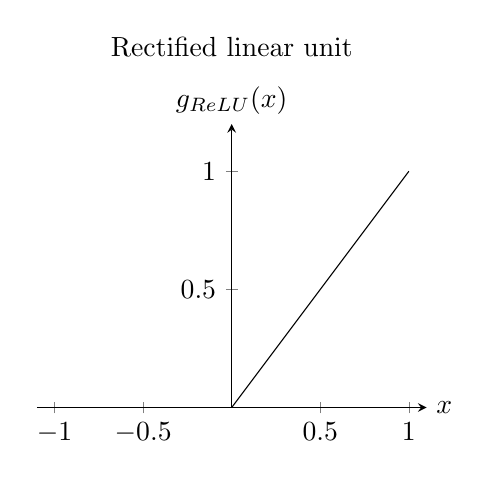
\begin{tikzpicture}
        \begin{axis}[
            x=2.25cm,
            y=3cm,
            axis lines=center,
            xlabel={$x$}, xlabel style={anchor=west},
            ylabel={$g_{\text{ReLU}}(x)$}, ylabel style={anchor=south},
            ymin=0, ymax=1.2,
            xmin=-1.1, xmax=1.1,
            samples=100,
            xtick={-1, -0.5, 0, 0.5, 1},
            ytick={0, 0.5, 1},
            title style={at={(0.5,1)},anchor=south,yshift=15.0},
            title={Rectified linear unit}
        ]
            \addplot[black][domain=0:1] {x};
            \addplot[black][domain=-1:0] {0};
        \end{axis}
    \end{tikzpicture}
    \caption{Plots of the the two most common activation functions.}
    \label{fig:activation_functions}
\end{figure}

Rectified units do not suffer from the \textit{vanishing gradient effect} \cite{glorot2011}.
This phenomenon occurs with sigmoid activation functions when they reach high saturation, i.e. when the input is significantly far from zero such that the gradient is almost horizontal.
However, the vanishing gradient problem is usually not prevelant in shallow\footnote{Shallow networks refer to ANNs with few layers.} networks so the sigmoid function still remains popular \cite{neal1992}.

\paragraph{ANNs as regression models}
We can employ an ANN to model a regression problem of the form given in (\ref{eq:reg_model}). 
To do so, we need at least $D+1$ neurons in the network. 
We consider the first $D$ units to be the \textit{input} neurons, and the last neuron, $n$, is the output unit.
Furthermore, we require $w_{j,k}=0$ for $j,k \in \mathbb{Z}^+$ where $j \leq n$ and $k \leq D$ to ensure that there are no links feeding into the input neurons.

To obtain the prediction $\hat{y}$ given the $D$-dimensional feature vector $\vec{x}$, we set the activation of the $i$th unit to the value the $i$th element in $\vec{x}$ for $i=1,\dots,D$.
Then, we propagate the activations using (\ref{eq:ann_activation}) until finally the prediction is the activation of the last neuron, $\hat{y}=a_n$.
This process is often called \textit{forward propagation} or \textit{forward pass} \cite{russell2010}.

\subsection{Single-layer network}
We introduce a single-layer network (SLN) as a type of ANN which consists of two conceptual layers, an input and an output layer.
Every input node is connected to every output node, but there are no intra-layer links (i.e. there are no links between any two input nodes or any two output nodes), as shown in Figure \ref{fig:single_layer_perceptron}. 
This is what we call a \textit{fully-connected feedforward} architecture.
SLN architectures will always form a \textit{directed acyclic graph} (DAG) because there are no intra-layer or backwards connections.

\begin{figure}
    \begin{center}
        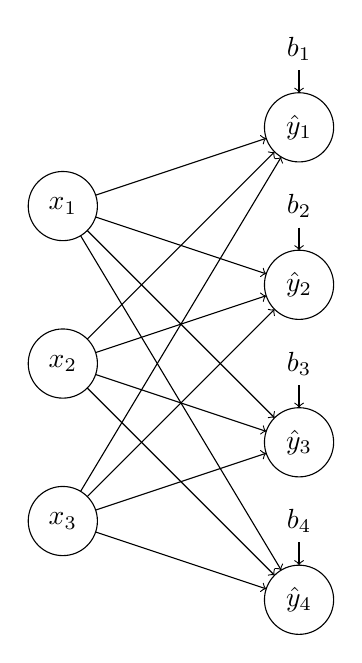
\begin{tikzpicture}
            [
                neuron/.style = {draw, circle, minimum size=25pt, inner sep=0pt, outer sep=0pt},
            ]
            \node [neuron] (x1) at (0,0) {$x_1$};
            \node [neuron] (x2) at (0,-2) {$x_2$};
            \node [neuron] (x3) at (0,-4) {$x_3$};
            \node [neuron] (n1) at (3,1)  {$\hat{y}_1$};
            \node [neuron] (n2) at (3,-1) {$\hat{y}_2$};
            \node [neuron] (n3) at (3,-3) {$\hat{y}_3$};
            \node [neuron] (n4) at (3,-5) {$\hat{y}_4$};
            \node (b1) at (3, 2) {$b_1$};
            \node (b2) at (3, 0) {$b_2$};
            \node (b3) at (3, -2) {$b_3$};
            \node (b4) at (3, -4) {$b_4$};
            \draw[->] (x1) -- (n1);
            \draw[->] (x1) -- (n2);
            \draw[->] (x1) -- (n3);
            \draw[->] (x1) -- (n4);
            \draw[->] (x2) -- (n1);
            \draw[->] (x2) -- (n2);
            \draw[->] (x2) -- (n3);
            \draw[->] (x2) -- (n4);
            \draw[->] (x3) -- (n1);
            \draw[->] (x3) -- (n2);
            \draw[->] (x3) -- (n3);
            \draw[->] (x3) -- (n4);
            \draw[->] (b1) -- (n1);
            \draw[->] (b2) -- (n2);
            \draw[->] (b3) -- (n3);
            \draw[->] (b4) -- (n4);
        \end{tikzpicture}
    \end{center}
    \caption{A single-layer perceptron with three input and four output neurons.}
    \label{fig:single_layer_perceptron}
\end{figure}

We purposefully use the term SLN instead of single-layer perceptron (SLP) to avoid confusion. 
A SLP has only one output unit and uses the threshold activation function given in (\ref{eq:thres_activation}) \cite{rosenblatt1958}.
In our definition of a SLN we allow more than one output and impose no restrictions on $g$, except that the same activation function is used for every output neuron.
We still use the term `single layer' because the input layer, lacking any incoming weight or bias connections, is not considered to be a `proper' layer.

Let us consider a SLN with $m$ inputs and $n$ outputs. 
Since every output unit $i$ only has connections from every input unit $j$,
we can adapt (\ref{eq:ann_activation}) to give the activation of a particular output neuron $i$ as
\begin{equation}
    a_i = y_i = g\left({ex}_i\right) = g\left(\sum_{j=1}^m{w_{j,i} x_j} + b_i\right)
    = g\left( \vec{w}_i\tran \vec{x}_i + b_i\right)
\end{equation}
where
$
    \vec{w}_i = \begin{bmatrix}
        w_{1,i} & w_{2,i} & \cdots & w_{m,i}
    \end{bmatrix}\tran
$
represents the weights of all the edges that connect to output unit $i$.
If we use the $m \times n$ matrix
\begin{equation}
    \vec{W} = \begin{bmatrix}
        \vec{w}_1 & \vec{w}_2 & \cdots & \vec{w}_n
    \end{bmatrix} = \begin{bmatrix}
        w_{1,1} & w_{1,2} & \cdots & w_{1,n} \\
        w_{2,1} & w_{2,2} & \cdots & w_{2,n} \\
        \vdots & \vdots & \ddots & \vdots \\
        w_{m,1} & w_{m,2} & \cdots & w_{m,n}
    \end{bmatrix}
\end{equation}
to capture all weights and the vector $\vec{b} = \begin{bmatrix}
    b_1 & b_2 & \cdots & b_n
\end{bmatrix}\tran$ for the biases, we can give a mathematical formula describing the relationship between the inputs and outputs as
\begin{equation}
    \label{eq:single_layer_perceptron}
    \vec{f_{\text{SLN}}}(\vec{x}; \vec{W}, \vec{b}, \vec{g}) = \vec{g}\left( \vec{W}\tran \vec{x} + \vec{b} \right).
\end{equation}
Unlike the formula for a regression model, this is a vector-valued function, due to the fact that there are multiple outputs. 

Note that when $n=1$, we reach the same form as in (\ref{eq:reg_model}). 
Moreover, if we additionally use the threshold activation function from (\ref{eq:thres_activation}), we arrive at the SLP model given by \citet{rosenblatt1958}.

\subsection{Multi-layer perceptron}
\label{sec:multi_layer_perceptron}
A multi-layer perceptron\footnote{Unlike SLPs, the activation function in a MLP as defined in literature does not necessarily need to be the binary threshold function $g_\text{thres}$; in fact, it is often one of the more modern activation functions explained in Section \ref{sec:activation_functions} \cite{hastie2017,burkov2019}. Hence we can use the term `multi-layer perceptron'.} (MLP) is a fully-connected feedforward ANN architecture with multiple layers which we will define in terms of multiple nested functions as in \citet{burkov2019}.
A MLP with $L$ layers is the mathematical function
\begin{equation}
    f_{\text{MLP}}(\vec{x})
        = \hat{y}
        = f_L \left(
            \vec{f}_{L-1} \left(
                \vec{\dots} \left(
                    \vec{f}_1 \left(
                        \vec{x}
                    \right)
                \right)
            \right)
        \right)
\end{equation}
where $\vec{f}_l(\vec{x}) = \vec{f_{\text{SLN}}}(\vec{x}; \vec{W}_l, \vec{b}_l, \vec{g}_l)$ for $l = 1, \dots, L-1$. 
In order to fully define a MLP, we need the three-tuple
\begin{equation}
    \label{eq:mlp_three_tuple}
    \langle \mathscr{W}, \mathscr{B}, \mathscr{G} \rangle
\end{equation}
where $\mathscr{W} = \vec{W}_1, \vec{W}_2, \dots, \vec{W}_L$ are the weight matrices, $\mathscr{B} = \vec{b}_1, \vec{b}_2, \dots, \vec{b}_L$ the bias vectors, and $\mathscr{G} = \vec{g}_1, \vec{g}_2, \dots, \vec{g}_L$ the vector-valued activation functions.
Notice that for every $l < L$, $\vec{W}_l$ is a $n_l \times m_l$ matrix such that $n_l=m_{l+1}$ to esnure that the number of outputs of layer $l$ is the number of inputs to layer $l+1$.
This means that the MLP has $m_1$ input neurons.
The outermost function $f_L$ is the scalar-valued function $f_L(\vec{x}) = f_{\text{SLN}}(\vec{x}; \vec{W}_L, \vec{b}_L, \vec{g}_L)$ because it represents a SLN with only one output unit which also means that $\norm{\vec{b}_L}=1$, $\vec{W}_L$ has only one row, and finally $n_L=1$.

The graph representing this type of network consists of connecting the outputs of the SLN representing layer $l$ with the inputs of the SLN representing layer $l+1$, as shown in Figure \ref{fig:multi_layer_perceptron}. 
The layers between the input and output layers are referred to as \textit{hidden} layers.

\begin{figure}
    \begin{center}
        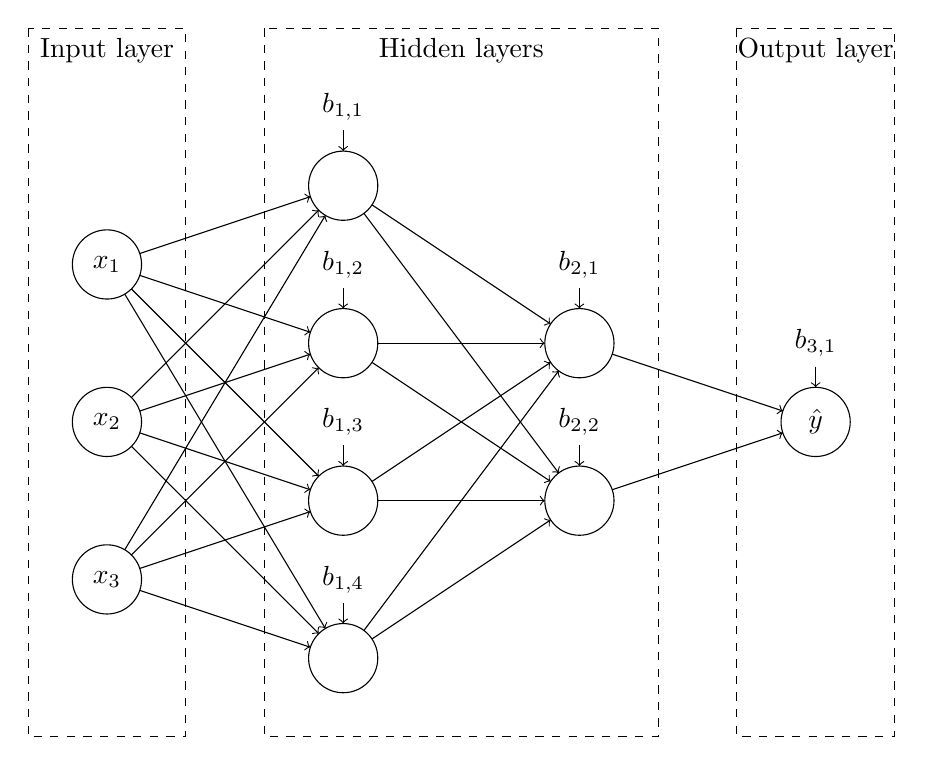
\begin{tikzpicture}
            [
                neuron/.style = {draw, circle, minimum size=25pt, inner sep=0pt, outer sep=0pt},
            ]
            \node [neuron] (x1) at (0,0) {$x_1$};
            \node [neuron] (x2) at (0,-2) {$x_2$};
            \node [neuron] (x3) at (0,-4) {$x_3$};
            \node [neuron] (h11) at (3,1) {};
            \node [neuron] (h12) at (3,-1) {};
            \node [neuron] (h13) at (3,-3) {};
            \node [neuron] (h14) at (3,-5) {};
            \node [neuron] (h21) at (6,-1) {};
            \node [neuron] (h22) at (6,-3) {};
            \node [neuron] (y) at (9, -2) {$\hat{y}$};
            \node (b11) at (3, 2) {$b_{1,1}$};
            \node (b12) at (3, 0) {$b_{1,2}$};
            \node (b13) at (3, -2) {$b_{1,3}$};
            \node (b14) at (3, -4) {$b_{1,4}$};
            \node (b21) at (6, 0) {$b_{2,1}$};
            \node (b22) at (6, -2) {$b_{2,2}$};
            \node (b3) at (9, -1) {$b_{3,1}$};
            \draw[->] (x1) -- (h11);
            \draw[->] (x1) -- (h12);
            \draw[->] (x1) -- (h13);
            \draw[->] (x1) -- (h14);
            \draw[->] (x2) -- (h11);
            \draw[->] (x2) -- (h12);
            \draw[->] (x2) -- (h13);
            \draw[->] (x2) -- (h14);
            \draw[->] (x3) -- (h11);
            \draw[->] (x3) -- (h12);
            \draw[->] (x3) -- (h13);
            \draw[->] (x3) -- (h14);
            \draw[->] (h11) -- (h21);
            \draw[->] (h11) -- (h22);
            \draw[->] (h12) -- (h21);
            \draw[->] (h12) -- (h22);
            \draw[->] (h13) -- (h21);
            \draw[->] (h13) -- (h22);
            \draw[->] (h14) -- (h21);
            \draw[->] (h14) -- (h22);
            \draw[->] (b11) -- (h11);
            \draw[->] (b12) -- (h12);
            \draw[->] (b13) -- (h13);
            \draw[->] (b14) -- (h14);
            \draw[->] (b21) -- (h21);
            \draw[->] (b22) -- (h22);
            \draw[->] (b3) -- (y);
            \draw[->] (h21) -- (y);
            \draw[->] (h22) -- (y);
            \draw[dashed] (-1,3) rectangle (1,-6);
            \draw[dashed] (2,3) rectangle (7,-6);
            \draw[dashed] (8,3) rectangle (10,-6);
            \node[below] (input) at (0,3) {Input layer};
            \node[below] (hidden) at (4.5,3) {Hidden layers};
            \node[below] (output) at (9,3) {Output layer};
        \end{tikzpicture}
    \end{center}
    \caption{A multi-layer perceptron with three inputs and two hidden layers.}
    \label{fig:multi_layer_perceptron}
\end{figure}

Since MLPs are simply nested SLNs, it follows that MLPs retain the DAG property and are therefore \textit{feedforward} networks as well.
In the forward pass, the activations are propagated from layer to layer (i.e. nested function to nested function) as in (\ref{eq:single_layer_perceptron}).



\chapter{Neural network learning}
\section{Gradient descent with mean squared error}
\section{Local minimum problem}
\section{Simulated annealing}

\chapter{Neural surfing theory}
\section{Weight and output spaces}
In Section \ref{sec:multi_layer_perceptron} we determined that we need the three tuple from (\ref{eq:mlp_three_tuple}) to fully define a MLP. 
Most importantly, we have $\mathscr{W} = \vec{W}_1, \vec{W}_2, \dots, \vec{W}_L$ and $\mathscr{B} = \vec{b}_1, \vec{b}_2, \dots, \vec{b}_L$ representing each layer's weight matrices and bias vectors, respectively. 

\paragraph{Weight space}
We define the weight space $\mathcal{W}$ of a MLP as the set of all possible assignments to its \textit{trainable parameters}. 
The trainable parameters are its weights and biases, so the weight space encompasses all possible configurations of $\mathscr{W}$ and $\mathscr{B}$. 

A SLN with $m$ inputs and $n$ outputs will have $m \times n$ weights and $n$ biases, totalling $n(m+1)$ trainable parameters.
Now consider a MLP with $L$ layers, where $m_1, m_2, \dots, m_L$ is the number of inputs to each layer. 
For any layer $l$, the number of outputs $n_l$ is $m_{l+1}$ except for the last layer where $n_L=1$.
It follows that the total number of trainable parameters in the network is
\begin{align*}
    P &= \sum_{l=1}^{L}{\left(n_l (m_l + 1)\right)} \\
    &= \sum_{l=1}^{L-1}{\left(m_{l+1} (m_l + 1)\right)} + m_L + 1,
\end{align*}
so the weight space for that network is defined as
\begin{equation}
    \mathcal{W} = \mathbb{R}^P.
\end{equation}

\paragraph{Output space}
The output space $\mathcal{O}$ spans the space of all possible output predictions on the training set.
In our definition of a MLP from Section \ref{sec:multi_layer_perceptron}, it states that the network must only have one output node and thus the prediction $\hat{y}$ is a scalar. 

From (\ref{eq:sup_learn_prediction}), the vector $\vec{\hat{y}}$ represents the prediction $\hat{y}$ for all $N$ training samples.
This means that the output space spans all possible assignments of $\vec{\hat{y}}$, so
\begin{equation}
    \mathcal{O}=\mathbb{R}^N.
\end{equation}

\paragraph{Relationship between weight and output spaces}
\todo

\chapter{Problems}
\section{Stripe problem}


\chapter{Generalising neural surfing}
Generalize to classification as regression with multiple output variables
